\documentclass[conference]{IEEEtran}
\usepackage{cite}
\usepackage{graphicx}
\usepackage{float}

\begin{document}

\title{GenegleBot: An Agent that Genetically Generates Concurrent Musical Accompaniment
	\\
	{\footnotesize }
}

\author{\IEEEauthorblockN{Gregory Hughes}
	\IEEEauthorblockA{\textit{Computer Science} \\
		\textit{WVU Tech }\\
		gshughes@mix.wvu.edu}
	\and
	\IEEEauthorblockN{Mardigon Toler}
	\IEEEauthorblockA{\textit{Computer Science} \\
		\textit{WVU Tech}\\
		mmtoler@mix.wvu.edu
	}
}

\maketitle

\begin{abstract}
	One of the most impressive feats of musical performance is improvising while playing with another musician. We present an Artificial Intelligence agent that emulates this feat by playing music alongside a real musician as if it were also another musician.
	While a simple melody is being played by a performer, the AI agent procedurally generates a simple melody using a genetic algorithm. The notes from the melody are stored in a custom data structure that reaches full capacity after 12 notes. As time passes, several possible accompaniments, called individuals, of the same size are randomly generated and then merged based on an evaluation of how well they sound when contrasted with the input melody. Using the genetic algorithm, the best-sounding individuals that synchronize with the input melody are more likely to be created. The best individual to emerge from multiple rounds of merging and the occasional mutation is then sampled for an output note while next notes are being recorded. The result after many iterations is a computer-generated melody that plays with the accompanying tune in harmony.
	There are existing programs that generate musical accompaniment, but the significance of this approach is its ability to generate music in real time during a musical performance, making it an interesting tool for use in both practice and performance.
	
\end{abstract}

\section{Introduction}

When musicians perform and practice, they may desire accompaniment. Performances involving multiple musicians may allow for much more complex, interesting music. While there are plenty of examples of solo musical performances, it is more common for musicians to work together when playing music. In addition, a musician may wish to have this sort of accompaniment even when other musicians are not available. Therefore, we wish to develop some way to utilize artificial intelligence as a means of producing accompaniment.  In the pursuit of finding an algorithm to aid in musical performances, certain benefits of artificial intelligence come to mind. While it is entirely possible for performers to play alongside pre-recorded pieces of music, doing so has its disadvantages. Pre-recorded music has the unfortunate likelihood of becoming stale after it is played many times, and musicians may wish to be able to improvise. Recordings would have no ability to adapt to this sort of behavior. 

An artificially intelligent agent may be able to create musical accompaniment based on the performance of musician.  A genetic algorithm is a type of artificial intelligence that may be applicable here. These algorithms work by creating a population of individuals, each of which has many chromosomes representing pieces of a proposed solution. Like in the natural process of macroevolution, these individuals can “reproduce” over time to replace the current population, and fitter individuals (those for which a problem-specific fitness function will have the largest relative output) stand a better chance of reproducing.  Individuals also have a random chance to mutate, an event which modifies their chromosomes unpredictably. Through the process of mutation, there is a chance that the agent’s output will vary from the user input, and these variations may still have a chance to remain fit enough to reproduce for future generations of the algorithm. This effect, along with pressure to stay somewhat similar to the user input, may result in an agent that is able to modify its behavior over time such that its current performance stays associated with the user’s performance while not simply parroting it.  It is this combination of musical accompaniment and genetic algorithms that is the defining aspect of our project. 

GenegleBot, pronounced “Jingle Bot”, is an rationally-acting artificial intelligence  agent created with the intention of playing music that adapts to user input.  The use of the term “rational” can be tricky since the topic is music, an inherently subjective concept.  There is no “best” possible choice to make when dealing with music.  Composing music rationally is usually comes down to making sure everything “sounds good” according to a predetermined and arbitrary definition of good.  GenegleBot’s fitness function, the process by which it evaluates collections of notes it chooses to play, is based on how often the notes it chooses appear in its input melody.  It generates several selections of possible notes to play and then fuses and alters those selections using a genetic algorithm.  Once the genetic process has iterated enough times, a note is chosen from the “fittest” selection of notes and is played.  With all this in mind, calling GenegleBot a rationally-acting agent seems reasonable.  It is, however, not the first of its kind.


\section{Existing Works}
One of the earliest works to describe the use of a genetic algorithm to compose music is “Bach in a Box: The Evolution of Four Part Baroque Harmony Using the Genetic Algorithm” by Ryan A. McIntyre \cite{b2}. Published in 1994, this article is about McIntyre's attempt to use artificial intelligence to compose Baroque-style music. He spends most of his Background section defining what made music from the Baroque period unique. He explains how music from that era was made up of multiple parts or voices that each have their own unique tune but also form chords when combined. Using a simple major-key soprano melody as input, McIntyre's program is able to accurately generate the alto, tenor and bass harmonies to create a basic Baroque-style composition. McIntyre also states that he is quite pleased with his results \cite{b2}. What makes his article noteworthy in this context, however, is how he formulated his fitness function.

McIntyre uses rules based on music theory to make his fitness function. Specifically he uses a set of seven functions that grade each individual in such a way that the sum of the best scores they could give equals 68 times the length of the individual. These functions are all based on concepts of music theory such as harmonic resolution, chord repetition, or a lack thereof depending on the context, and contrary motion. There are two functions, one based on chord formation and one based on the space between tunes, the take higher precedence over the other five. What this means is that an individual must score high enough on these two rubrics before it can be judged further \cite{b2}.  This practice of devising fitness functions based music theory is one that is still in use today.

”Polyphonic accompaniment using genetic algorithm with music theory”, written by Chien-Hung Liu and Chuan-Kang Ting and published in 2012. describes an agent that was designed to create polyphonic accompaniment for a piece of music by applying a genetic algorithm\cite{b1}.  Unlike “Bach in a Box”, which composed it’s own music, Liu and Ting’s AI was focused on providing main accompaniment, bass accompaniment, and chord accompaniment\cite{b1}. In their implementation, the genetic algorithms for these three pieces of accompaniment were performed one after another, getting feedback from previous results. That is, the accompaniment output from one genetic algorithm is part of the input for the next genetic algorithm.

Liu and Ting’s fitness function takes musical sections as input and examines it for various features, each of which has a corresponding weight assigned to it. For example, the presence of a perfect fifth interval in the input (for main accompaniment) causes that chromosome to be awarded with +15 fitness. On the other hand, a feature such as the presence of a no chord notes (in an individual for bass accompaniment) will result in the fitness being reduced by 20. A table of weights are provided by McIntyre for each of the different stages of generation accompaniment. That is, different features of an individual will be judged differently depending on which type of accompaniment is being generated.  It is evident that music theory is a venerable basis for fitness functions in music-based genetic algorithm but since GenegleBot is meant to play in real-time, it requires something faster.

\section{Project Overview}

The primary differences between our genetic music algorithm and the GA proposed in \cite{b1} are data structures used to represent musical information and the user interface. While the GA by Liu and Ting computes a musical accompaniment given an entire section of music as an input, our artificial intelligence is designed to be operated in real time during a performance. In addition, our genetic algorithm models the performance by maintaining a FIFO queue of recently input notes and maintains a histogram of this queue. This queue serves as an individual's chromosome.  This input histogram is used directly as the input to the genetic algorithm's fitness function; that is, each individual is ranked based on the similarity between its own proposed histogram and the input histogram.
The representation implemented by Liu and Ting relies on storing musical sections as a whole in data structures\cite{b1}.  Our implementation always stores a number of the most recently input notes, regardless of musical section. The differences between these data structures relate to differences in the motivations of the fitness functions. Our fitness function increases as an individual's histogram becomes more similar to the histogram of the input. In contrast, the fitness function of Liu and Ting is comprised of rules inspired by music theory. Their AI's chromosomes are judged by their compliance to these rules\cite{b1}.
In addition to the different data structures, the dissimilarities also extend to the interface. As our genetic algorithm is meant to provide accompaniment while the user is playing music, all fitness functions are computed only with the knowledge of the recent portion of a performance. The Music Theory fitness function of Liu and Ting, however, is not limited to only a recent performance history but may consider large musical sections, as the output of their genetic algorithm is meant to be computed for an entire pre-recorded performance. 

Our fitness function is computed for each individual
$x_{i} \in \{x_{1},x_{2},...,x_{n}\} $ where $n$ is the population size, using
a vector of recent input, $\vec{y}$, and a vector $\vec{z}$. Each element of these
vectors corresponds to a certain note on a piano keyboard, and the value of
each element represents how often that note occurs in a signal. Thus, each vector
can be thought of as a histogram of notes. The fitness of an individual $\vec{v}$ is given by:
\[ Fit(\vec{v}) = \vec{v}\cdot\vec{y} \]
\[  = \sum_{i=1}^m \vec{v}_{i}\vec{y}_{i} \]
where $m$ is the number of elements (notes) in the vectors. This can be thought of as the "likeness" of an individual's histogram to
the input histogram. It should be noted that due to the nature of this fitness function, the order in which the most recent notes are played has no effect.

The “environment” of this agent consists of the user input queue as well as timing information. The agent’s sensor and actuator are MIDI input and output ports. In order for the agent to perceive time passing, it relies on sensing MIDI Beat Clock messages. Also, in order to populate the user input queue, it relies on MIDI Note On messages being routed to its input port. Another part of the agent’s environment is the agent itself; the result of each generation of the genetic algorithm will change the population and therefore affect the result of future generations. The agent’s output consists also of MIDI Note On messages so that it may interact with hardware or software to produce audio. Our specific implementation in C used the JACK Audio Connection Kit server to facilitate sensing and sending MIDI messages and receives its MIDI. Currently, the agent always assumes that the user’s melody is being played in the 4/4 meter. A digital audio workstation is used to produce a MIDI Beat Clock signal.

As the agent perceives time passing, it will periodically simulate generations of the genetic algorithm, from which a fit individual is selected. It is important to note that during the mutation process in the current implementation, an individual's histogram has notes removed randomly until it is of small size so that the output histograms remain more dense. This individual’s histogram of notes is then sampled to produce the next note of output. As an example, suppose that the most fit individual has a histogram representing two C notes and one E note. Then, if it is time for the agent to produce its next note of output, it will have a 2/3  chance of selecting C and a 1/3 chance of selecting D.  During normal operation, the genetic algorithm simulates three generations during every 8th note interval (sensed from the MIDI Beat Clock input). However, to collect the data for this experiment, each simulation occurs immediately after every input note (which would be equivalent to the user entering input twice every beat). 


\section{Experiments and Results}

    In order to evaluate GenegleBot's performance we need to know how "fit" it's output histograms are in different circumstances.  As previously stated, how fit a histogram is depends on how often the m most recent notes in the input appear in that histogram.  To keep each test consistent, we formulated three sample melodies with 12 notes each.  For each sample input, we performed 30 simulations of the genetic algorithm, in which each simulation consisted of 3 generations. We recorded the maximum fitness for the most fit individual after each of these simulations, from which we could calculate the average fitness achieved for a sample input as well as measuring how the fitness was distributed for every sample input. In our specific configuration, the maximum size of the user input was $ m=12 $. 
    
Three sample inputs were used: 4 D minor triads, an arpeggio in C, and finally a chromatic scale. Because of the repetition in the first sample input, we expected individuals to be able to achieve higher fitness because of the user input histogram being more dense in fewer bins. In contrast, we expected the chromatic user input to cause the minimal possible fitness, because the user input histogram was as sparse as possible. 

For the first sample input consisting of 4 repeated D minor triads, the data was distributed as shown in Figure \ref{fig:dminordist}, with a maximum fitness score of 12 and an average fitness score of 8.8. 


\begin{figure}[H]
	\centering
	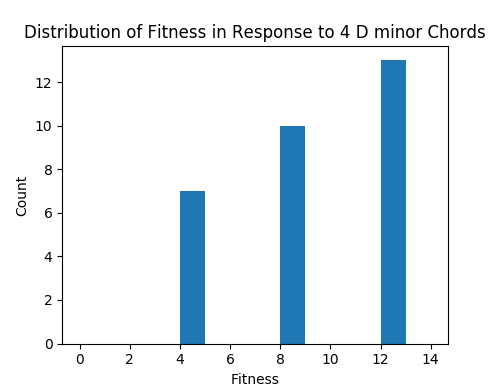
\includegraphics[width=0.8\linewidth]{dMinorDist}
	\caption{}
	\label{fig:dminordist}
\end{figure}


Next, the input of a melody in C consisting of the notes (C, D, E, F, G, A, B, C, C, E, B, C), resulted in the distribution of fitnesses in Figure \ref{fig:cmelodydist}, with a maximum fitness score of 12 and an average fitness score of  approximately 6.12. 


\begin{figure}[H]
	\centering
	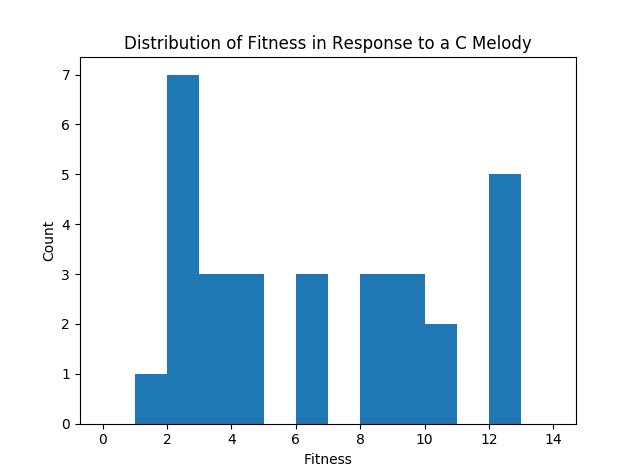
\includegraphics[width=0.8\linewidth]{cMelodyDist}
	\caption{}
	\label{fig:cmelodydist}
\end{figure}

Finally, for the user input consisting of the chromatic scale (which results in the user input histogram having a uniform distribution), the best individuals' fitnesses had the distribution shown in Figure \ref{fig:chromaticdist}. The maximum and average fitness score achieved was 3.


\begin{figure}[H]
	\centering
	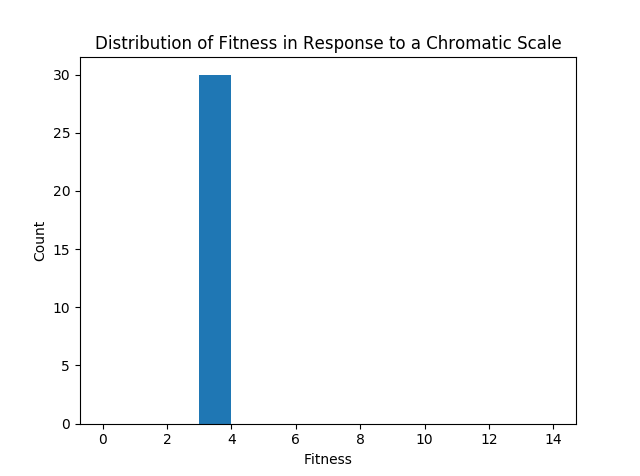
\includegraphics[width=0.8\linewidth]{chromaticDist}
	\caption{}
	\label{fig:chromaticdist}
\end{figure}

This data seems to confirm our suspicion that the agent will not perform well if the user input is extremely varied (like in the case of the purely chromatic input). To coax good performance from the agent, the user input must be somewhat repetitive or at least consist mostly of notes that you would be okay with the agent outputting. Our agent is incapable of doing any kind of inference about what key the user is performing in. Therefore, a good output relies entirely on the input consisting mostly of notes that would also sound good as output.




%In Figure \ref{fig:dminordist} you can see.
%In Figure \ref{fig:cmelodydist} there is stuff.

\section{Conclusion}

The question driving the creation of GenegleBot was: "Can a genetic algorithm be used to create real-time musical accompaniment?" Previous articles about how music and genetic algorithms work together could not provide a clear answer because they were usually either about composing music independent from user input or generating harmonies based on an already completed melody.  However, the results from the experiments performed with GenegleBot seem to point to the answer being "yes."  While the agent itself is limited to only one type of meter and the structure of the input, the accompaniment it produces matches up well with input that adheres to these limitations.  Furthermore, it is feasible for GenegleBot or similar agents to overcome these limitations given enough time and effort. There are various improvements we are already aware of that this agent may improve from if they were implemented, such as analysis of (and adaptation to) the rhythmic properties of the user input. Another possible improvement could be made by allowing a user to configure different properties of the agent, such as maybe specifying "bad" notes, for which an individual's fitness could be reduced for including in its histogram. With these, along with other possible improvements, AI could potentially be good enough at producing original music to be viable as accompaniment during live, professional performances.

\begin{thebibliography}{1}
	
	\bibitem{b1}
	Chien-Hung Liu and Chuan-Kang Ting, "Polyphonic accompaniment using genetic algorithm with music theory," 2012 IEEE Congress on Evolutionary Computation, Brisbane, QLD, 2012, pp. 1-7.
		
	\bibitem{b2}
	A. McIntyre, "Bach in a box: the evolution of four part Baroque harmony using the genetic algorithm," Proceedings of the First IEEE Conference on Evolutionary Computation. IEEE World Congress on Computational Intelligence, Orlando, FL, 1994, pp. 852-857 vol.2.
			
	
	
\end{thebibliography}

	
\end{document}

